\documentclass[12pt]{article}
\usepackage[a4paper,margin=25mm]{geometry}
\usepackage{fontspec}
\usepackage{unicode-math}
\setmainfont{lmroman10-regular.otf}[
  BoldFont=lmroman10-bold.otf,
  ItalicFont=lmroman10-italic.otf,
  BoldItalicFont=lmroman10-bolditalic.otf]
\setsansfont{lmsans10-regular.otf}[BoldFont=lmsans10-bold.otf]
\setmonofont{lmmono10-regular.otf}[Scale=MatchLowercase]
\setmathfont{latinmodern-math.otf}
\usepackage{microtype}
\usepackage{amsmath}
\usepackage{graphicx}
\usepackage{booktabs}
\usepackage{array}
\usepackage{pdflscape}
\usepackage{xcolor}
\usepackage{lineno}
\usepackage{cite}
\usepackage[hidelinks]{hyperref}
\usepackage{caption}
\captionsetup{font=small,labelfont=bf}
\setlength{\parindent}{0pt}
\setlength{\parskip}{0.55em}
\setlength{\emergencystretch}{2em}
\renewcommand{\familydefault}{\rmdefault}
\definecolor{placeholder}{HTML}{FFF2A8}


\title{Probabilistic graph completion of historical Chinese incense formulas under source shift}

\author{\colorbox{placeholder}{[Author name]}\\\colorbox{placeholder}{[Affiliation, city, country]}\\\colorbox{placeholder}{[Corresponding email]}}

\date{}

\begin{document}

\maketitle

\linenumbers

\begin{abstract}

Historical incense books preserve formulas unevenly, while modern odor datasets describe molecules and rarely recipes. We formulate missing-ingredient recovery as source-shifted probabilistic set completion. Xiangji-CGIR combines a directed material graph with Bayesian inclusion, ingredient-count and composition models. We curated 91 family-unique Chinese incense formulas from six work groups. At 50\% observed context, the graph reached source-macro hidden-component F1 0.379 versus 0.338 for frequency, 0.343 for formula k-nearest neighbours and 0.334 for PureSVD. Removing nine cross-work high-similarity formulas retained the graph advantage, 0.348 versus 0.322. Development-calibrated count intervals achieved 0.825 coverage at nominal 0.80. The full decoder reached F1 0.377, and confirmation on a quarantined work reached 0.577. An 18-material chemical kernel did not improve completion. Co-formulation structure transfers across texts; molecular similarity alone does not represent historical ingredient complementarity.

\end{abstract}

\section*{Introduction}

Smell can carry cultural meaning, but it leaves a fragmented archive. Heritage frameworks now treat historic odors as objects that can be identified, described and preserved \cite{ref1}. The Odeuropa data model connects odor sources, emissions, experiences, places and historical language \cite{ref2}. Analytical heritage science has also reconstructed the present smell of a surviving perfume residue by combining gas chromatography, olfactory detection and sensory validation \cite{ref3}. Historical incense formulas pose a different computational problem. The material may no longer survive, and the books may preserve only a name, partial recipe, attributed source or literary description, with no measurable headspace sample.

Computational olfaction has learned useful mappings from molecular structure or mass spectra to perceptual descriptors \cite{ref4,ref5,ref6,ref7,ref8}. Mixture models now predict descriptors for pairs of aroma chemicals \cite{ref9}, and inverse design can optimize modern essential-oil mixtures against a requested scent profile \cite{ref10}. These systems start from molecules, spectra or controlled vocabulary. They do not recover a historical natural-material formula from incomplete evidence transmitted through different texts. Historical language processing addresses orthographic variation and sparse annotation \cite{ref11}, while recipe information extraction resolves ingredients and quantities from modern text \cite{ref12}. Neither line of work supplies a source-shifted benchmark for historical formula completion. Nearest-neighbour retrieval and low-rank recommendation test whether a historical graph adds information beyond local formula analogy or latent co-occurrence \cite{ref16,ref17}. Development-held-out interval expansion tests whether its count uncertainty transfers \cite{ref18}.

We define a formula as a sparse set of aromatic materials with relative dry-mass ratios. Given its title, source identifier and a known subset of ingredients, the task is to recover the hidden materials and their proportions. This setting tests a practical scholarly operation: completing a damaged or selectively transmitted formula from patterns learned in other works. It also exposes the central statistical difficulty. Incense vocabularies are long-tailed, formula sizes vary, and source traditions differ. A random record split would let near-identical textual and material conventions leak across training and test sets.

Xiangji-CGIR makes four contributions. First, it introduces a provenance-rich reference set of 91 family-unique formulas from six Chinese incense work groups, with stable source locators, canonical material identifiers and source-blocked splits. Second, it represents each formula as a hyperedge and converts training-only co-occurrence counts into a directed posterior-predictive material graph. Third, it couples that graph to a Gaussian-prior logistic inclusion decoder, an explicit ingredient-count posterior and a simplex-valued composition posterior. Fourth, it measures the contribution of chemistry through development ablations, an auxiliary inverse-odor task and shuffled material-chemistry assignments. Co-formulation structure transfers across historical works; title and source channels add no reliable gain beyond the graph, and pairwise chemical similarity does not improve completion.

\section*{Results}

\subsection*{A source-blocked benchmark exposes material and document sparsity}

The curation pipeline screened 120 candidate formulas and retained 91 with complete aromatic quantities. Each retained record links a verbatim transcription to a stable revision URL and locator. The six work groups contributed 38, 29, 10, 6, 6 and 2 formulas, respectively (Fig. 2a; Supplementary Table S1). The corpus contains 81 canonical aromatic materials. Formula size ranges from 2 to 17 materials, with a median of 6 and a mean of 6.85 (Fig. 2b). Thirty materials occur in one formula, while four materials appear in more than 40 formulas. This frequency profile makes rare-material recovery a defining part of the task, not a peripheral edge case.

Six formulas attributed to the Hong Xiangpu work group were removed before any model-facing statistic was constructed. The other 85 formulas from five work groups contain 80 materials and formed development and primary evaluation data. Ten primary folds held out every pair of work groups and trained on the remaining three. This design tests transfer to documents whose lexical and compositional habits are absent from training. Eighty-four formulas remained evaluable with at least two in-vocabulary components; one Huizhai formula did not.

\subsection*{A directed material graph carries the cross-document gain}

At the registered 50\% observation fraction, the global-frequency baseline reached source-macro hidden-component F1 0.338 and weighted Jaccard 0.378. Weighted Jaccard measures the fraction of total formula mass shared by the reference and prediction. The directed graph reached F1 0.379 and weighted Jaccard 0.390. The locked full decoder reached F1 0.377 and weighted Jaccard 0.390 (Fig. 3; Supplementary Table S2). Its mean work-level F1 difference from frequency was 0.0278. Four of five work groups improved; the source-bootstrap interval was [0.0079, 0.0473], while the exact five-block sign-flip test gave p = 0.125. Five independent work groups produce a coarse exact p-value grid, so the effect magnitude and cross-source pattern are the informative quantities.

The full decoder and graph-only scores were nearly identical. Their mean work-level F1 difference was 0.0010, the source-bootstrap interval was [\ensuremath{-}0.0072, 0.0100], and the exact sign-flip p-value was 0.875. Title similarity and source prevalence therefore did not add stable information after the observed ingredients reached the conditional graph. The graph is the effective model component.

Transfer varied by source. The full decoder reached hidden F1 0.443 on Liexiang Xinpu, 0.396 on Chen Xiangpu, 0.392 on the Xiangcheng compilation, 0.392 on Xiaolu Xiangpu and 0.210 on Huizhai Xiangpu (Fig. 3a; Supplementary Table S3). Weighted Jaccard ranged from 0.324 to 0.446. Reporting only the pooled mean would conceal this document effect.

After freezing the decoder, we added two competitive set-completion baselines with configurations selected on the five development work splits. Formula k-nearest neighbours reached primary hidden F1 0.343 and PureSVD reached 0.334, compared with 0.379 for the directed graph (Fig. 6a; Supplementary Table S10). The graph exceeded formula k-nearest neighbours by 0.0223 F1 and PureSVD by 0.0311 at the work level. Formula k-nearest neighbours produced the highest weighted Jaccard, 0.443, because it fixed supplied ratios and interpolated neighbour compositions. Applying the same mass constraint to the full decoder increased weighted Jaccard from 0.390 to 0.427 without changing its selected materials.

Nine formulas had aromatic material-set Jaccard at least 0.8 with a formula from another work group. Removing all nine reduced graph F1 to 0.348 and frequency F1 to 0.322; the graph retained a 0.0259 work-level advantage (Fig. 6b; Supplementary Table S11). High-similarity transmission therefore raises absolute performance but does not account for the graph-frequency ordering.

\subsection*{Context amount changes the residual task}

When 25\% of a formula was observed, graph-only reached hidden F1 0.408, compared with 0.388 for frequency and 0.400 for the full decoder. At 50\%, the values were 0.379, 0.338 and 0.377. At 75\%, they were 0.262, 0.237 and 0.263 (Fig. 4a; Supplementary Table S4). Hidden F1 falls as the observed fraction rises because the remaining labels form a smaller and harder residual set. At the sparsest 25\% context, graph-only beat the full decoder in all five work groups. The full model's extra channels dilute the strongest signal when little context is available.

Training frequency set a sharp recovery frontier. Hidden-material recall was 0.573 for materials appearing in at least five training formulas, 0.056 for those appearing two to four times, 0.023 for singletons and zero for out-of-vocabulary materials (Fig. 4b; Supplementary Table S5). The model most often overpredicted sandalwood, borneol, musk, agarwood and clove. Frequent misses included scrophularia root, spikenard, zhan-grade agarwood, frankincense and clove. Across five deterministic masks, the mean Jaccard similarity between predicted sets was 0.644. The error profile points to data coverage, not decoder depth, as the present performance ceiling.

\subsection*{Posterior outputs are useful but high probabilities remain overconfident}

Across 95,210 hidden candidate decisions, the locked decoder produced a Brier score of 0.0429 and expected calibration error of 0.0236. Those aggregate values are dominated by the large low-probability class. The reliability curve shows close agreement below probability 0.3 and increasing overconfidence above 0.4; the highest bin had mean probability 0.931 and empirical inclusion frequency 0.565 (Fig. 5a; Supplementary Table S6).

The formula-size posterior underestimated total ingredient count by 0.883 materials on average. Its mean absolute error was 1.190, and the nominal central 80\% interval covered 64.2\% of true counts. Work-held-out development residuals set a one-material expansion without accessing primary labels. The expanded interval covered 82.5\% in primary evaluation, while mean width increased from 1.24 to 2.86 materials (Fig. 6c; Supplementary Table S12). Conditional on the decoder selecting a true material, the 80\% Dirichlet ratio interval covered 91.2\% of its reference ratios. The selected set contained 63.1\% of all true components. Inclusion probabilities were accurate at low scores, count uncertainty required calibration and ratio intervals were conservative after correct selection.

\subsection*{Chemistry tests separate similarity from co-formulation}

Ratio estimation uses compositional-data geometry \cite{ref19}, compounds use radius-2, 2,048-bit Morgan fingerprints \cite{ref20}, and the implementation uses scikit-learn \cite{ref21}. The chemical evidence layer links 18 of 81 materials to 18 specimen-level analytical profiles drawn from 17 publications \cite{ref22,ref23,ref24,ref25,ref26,ref27,ref28,ref29,ref30,ref31,ref32,ref33,ref34,ref35,ref36,ref37,ref38} and 40 PubChem compounds. Each profile retains taxon, plant part, preparation, analytical method and measurement basis. The model also includes physicochemical descriptors and controlled odor tags. A pairwise kernel combines fingerprint Tanimoto similarity, positive physicochemical cosine similarity and positive odor-tag cosine similarity.

The best chemistry-enabled primary-task variant reached development F1 0.3905, compared with 0.3911 for the selected non-chemistry variant. Chemistry was therefore disabled before primary evaluation. The auxiliary odor-to-formula task used 44 legacy formulas and nested leave-one-family-out validation. Odor k-nearest neighbors reached pooled weighted Jaccard 0.2913. The forward-consistent model reached 0.2824, its no-chemistry ablation 0.2835 and shuffled chemistry 0.2863. Pairwise chemical resemblance did not encode historical co-formulation. Similar materials can substitute for one another, while formulas often combine chemically dissimilar materials for contrast, volatility control or processing behavior.

\subsection*{Quarantined-source confirmation reproduces the ranking}

After the model and analysis code were frozen, all 85 development formulas were used to predict the six Hong-source formulas. At 50\% observed context, frequency reached hidden F1 0.469, graph-only 0.558 and the full decoder 0.577 (Fig. 5b; Supplementary Table S7). Weighted Jaccard values were 0.420, 0.456 and 0.468. The full decoder exceeded frequency by 0.108 F1 across the six formulas. These records share one work group, so they confirm transfer to a new source without adding a sixth independent block to the primary inference.

A fixed case-selection rule chose the seed-17 confirmation formula closest to the six-formula median hidden F1. For \emph{Yinxiang fa}, six of eleven reference materials were observed. The decoder recovered zhan-grade agarwood, borneol and sandalwood; it missed frankincense and licorice and added clove and linglingxiang. Ingredient count was exact, hidden F1 was 0.600 and mass-constrained weighted Jaccard was 0.483 (Supplementary Table S8). This case shows the intended use of the ranking and its current failure mode: common structural partners are recoverable, while low-frequency components remain difficult.

\subsection*{The complete model runs on ordinary hardware}

Training the locked decoder on all 85 development formulas and 80 materials took a median 0.115 s across 11 serial repetitions on an Apple arm64 system. A prediction with 200 posterior samples took 1.70 ms. The interquartile ranges were 5.28 ms for fitting and 0.14 ms for prediction. The conditional graph uses dense O(NM\ensuremath{{}^{2}}) construction in the reference implementation, although sparse hyperedge accumulation reduces this to O(\ensuremath{\Sigma}\ensuremath{_{i}}|S\ensuremath{_{i}}|\ensuremath{{}^{2}}). With D decoder features and R training masks, logistic fitting uses RNM candidate rows and O(RNMD) work per objective evaluation. The small-data design keeps the full pipeline reproducible on a laptop.

\section*{Discussion}

Historical formula completion is tractable when partial ingredients survive and related source traditions provide repeated material structure. The directed graph improved hidden-component F1 over frequency across four of five work groups, exceeded formula-neighbour and low-rank baselines, survived removal of nine high-similarity formulas and reproduced its ordering on the Hong confirmation source. Conditional co-formulation is the transferable signal. Generic text features and the tested chemical kernel added no stable gain.

The model's strongest feature is also its simplest. For every observed material, the graph estimates a smoothed conditional distribution over candidate partners using training formulas only. Averaging these directed conditionals captures asymmetric recipe logic. Musk may strongly predict a common base material even when the reverse conditional is weaker. Bayesian multi-label models have previously exploited label co-occurrence under sparse supervision \cite{ref13}; Xiangji places that principle inside a document-held-out historical benchmark and joins it to explicit formula-size and composition posteriors. The source-blocked protocol follows the machine-learning requirement that deployment domains remain outside training data \cite{ref14}. Each historical work defines a domain in this study.

The negative chemistry result sharpens the theory. Molecular odor models \cite{ref4,ref5,ref6,ref7,ref8} and blend predictors \cite{ref9} learn perceptual similarity or descriptor response. Historical ingredient pairing is a complementarity relation. A sandalwood base and a volatile top note may be valuable together because they differ in molecular composition and evaporation behavior. The symmetric kernel collapses substitution and complementarity into one number. A stronger chemistry-aware model should represent directed functional roles and interactions: base versus modifier, volatility ordering, combustion products, odor thresholds and nonlinear mixture suppression. It should train against new formula sources or physical measurements, leaving the present confirmation work untouched.

The task also differs from two adjacent forms of olfactory reconstruction. GC-MS/O can recover odor-active compounds when a physical residue survives \cite{ref3}. Descriptor-to-mixture optimization can design a modern scent that matches a requested profile \cite{ref10}. Xiangji completes a recorded material formula from documentary structure. Its output is a candidate formula completion; sensory identity requires analytical and panel validation. The task is computationally testable because known formulas can be masked and transferred across sources.

Three limitations set the next experimental agenda. The corpus has five primary source blocks, one confirmation block and a long tail of materials supported by one or two formulas. One curator performed the current canonicalization; independent recuration must test label stability. The model has no combustion or sensory measurements, and the evaluated task assumes that part of the ingredient set is known. A second release should add independently annotated work groups, controlled burn-headspace profiles and ranked expert judgments. Those additions would support full text-to-candidate reconstruction while preserving the current benchmark.

The study establishes a rigorous computational baseline for historical-formulation research. It provides the dataset structure, leakage controls, uncertainty decomposition and negative controls needed to compare stronger models. Across source shift, learned recipe relations carry usable information, while chemical similarity must be modeled as interaction before it can guide historical ingredient pairing.

\section*{Methods}

\subsection*{Corpus construction and provenance}

We extracted formula candidates from public-domain Chinese incense texts and their Wikisource transcriptions. Each candidate stored the work and edition identifier, formula title, verbatim source span, stable revision URL, line locator, transcription hash, material mentions, quantity strings, process mentions and rights statement. The curation protocol separated aromatic materials from binders, liquids and processing aids. It converted historical mass expressions to qian on a relative basis, summed repeated mentions and normalized aromatic mass to one. Records with an unresolved aromatic quantity, list boundary or formula identity were excluded without imputation.

Canonicalization mapped material mentions to an ontology identifier while retaining the surface form and identity status. Grade terms for agarwood remained separate identifiers. Four contextually resolved characters carry explicit resolution records. Candidate families were compared by normalized title, material-set overlap, ratio pattern and source genealogy. One checked representative was retained per provisional family. The resulting version 0.1 reference set contains 91 formulas; 29 screened candidates were excluded. All transformations are executable and hash checked.

\subsection*{Prediction task and observation mechanism}

For formula i, let S\ensuremath{_{i}} be its aromatic material set and \textbf{w}\ensuremath{_{i}} \ensuremath{\in} \ensuremath{\Delta}\textasciicircum{}(M\ensuremath{-}1) its normalized composition over M canonical materials. The model receives title t\ensuremath{_{i}}, work identifier d\ensuremath{_{i}} and an observed subset O\ensuremath{_{i}} \ensuremath{\subset} S\ensuremath{_{i}} with the original ratios for those materials. It predicts S\ensuremath{_{i}} \textbackslash{} O\ensuremath{_{i}} and a complete composition.

We generated O\ensuremath{_{i}} deterministically from a cryptographic hash of formula identifier, observation fraction and seed. For a formula containing K materials, the mask retained min(K\ensuremath{-}1, max(1, round(fK))) materials, where f \ensuremath{\in} \{0.25, 0.50, 0.75\}. This rule guarantees at least one observed and one hidden in-vocabulary material. The registered primary fraction was 0.50. Five seeds, 17, 29, 43, 71 and 101, changed the observed subset but not the source splits.

\subsection*{Source-blocked splits}

The Hong work group and its six formulas were removed before vocabulary construction, prior estimation, feature scaling or model selection. Development used five leave-one-work-out folds. Primary evaluation used all ten unordered pairs of the five remaining work groups as test domains, with the other three groups as training data. Family identifiers were disjoint because the reference set contains one representative per checked family. Each test formula appears in four source-pair folds and five mask seeds. We first averaged repeated predictions for a formula, then averaged formulas within a work group, then averaged the five work groups. The historical work is the unit of primary inference.

\subsection*{Directed posterior-predictive material graph}

Each training formula defines a hyperedge over its aromatic materials. Let c\ensuremath{_{i}} denote the number of training formulas containing material i, c\ensuremath{_{i}}\ensuremath{_{j}} the number containing both i and j, and \ensuremath{\pi}\ensuremath{_{j}} = (c\ensuremath{_{j}} + 0.5)/(N + 1) the smoothed global prevalence of candidate j among N training formulas. The directed edge is

\[G_{ij}=\frac{c_{ij}+\alpha\pi_j}{c_i+\alpha},\]

with \ensuremath{\alpha} = 2. For an observed set O, graph affinity for candidate j is the arithmetic mean |O|\ensuremath{{}^{-}}\ensuremath{{}^{1}} \ensuremath{\Sigma}\ensuremath{_{i}}\ensuremath{\in}O G\ensuremath{_{i}}\ensuremath{_{j}}. Direction matters because G\ensuremath{_{i}}\ensuremath{_{j}} generally differs from G\ensuremath{_{j}}\ensuremath{_{i}}. During training, the graph for formula i was rebuilt without that formula, preventing its target labels from contributing to its own features.

\subsection*{Inclusion decoder}

The full feature vector for candidate j comprised global prevalence log odds, source-prevalence deviation, character n-gram title similarity, graph affinity, an observed-material indicator and observed log ratio. Odor-target channels were zero in the primary task because the reference formulas contain no independent odor observations. Chemistry channels were disabled in the locked model after development selection.

We standardized features on the training fold and fit a Gaussian-prior logistic model. The coefficient prior variance was C = 3.0, selected in development. Class-balanced likelihood weights prevented the absent-material class from dominating optimization. We restored population probabilities with the corresponding case-control prior-odds correction. A Laplace approximation at the maximum a posteriori estimate supplied a Gaussian coefficient posterior. Posterior predictive inclusion probabilities used a logistic-normal moment approximation; 80\% inclusion intervals came from coefficient draws. A separate 20,000-step Metropolis-Hastings check on a synthetic problem produced mean absolute predictive difference 0.0016 from the Laplace implementation.

All global prevalence, source prevalence and title-centroid features used leave-one-formula-out values for training examples. The title encoder used character 1- and 2-gram TF-IDF. Observed materials were forced into the output set after prediction.

\subsection*{Ingredient count and composition posteriors}

We modeled ingredient count separately because inclusion scores rank materials but do not determine where the ranked list should stop. We estimated a smoothed empirical distribution over total ingredient count from each training work, shrunk toward the global count distribution. At prediction time this distribution was conditioned on the exact deterministic masking rule and the observed material count. The posterior median selected formula size because absolute count error was the registered loss.

For selected materials, ridge regression predicted log ratios from the candidate feature vectors. Exponentiation and closure mapped those values to the simplex. We estimated a Dirichlet concentration from training log-ratio residual variance and drew 200 samples per evaluation prediction. Posterior means supplied reported ratios; 10th and 90th percentiles formed 80\% intervals. The final mass-constrained output holds every supplied ratio fixed and closes predicted hidden ratios to the remaining mass. This correction changes neither material ranking nor selection. We evaluated composition with weighted Jaccard, union-support ratio mean absolute error and Aitchison distance \cite{ref19}.

The original count interval used the 10th and 90th percentiles of the masked count posterior. We calibrated its width from the five leave-one-work-out development folds \cite{ref18}. For each development prediction, nonconformity was the integer distance from the true count to the original interval, or zero when covered. The finite-sample 80\% quantile over 420 development predictions was one material. We expanded both primary interval endpoints by that value, retaining at least one hidden component. Primary labels did not determine the expansion.

\subsection*{Chemoinformatic evidence layer}

Targeted searches identified analytical studies for materials in the ontology \cite{ref22,ref23,ref24,ref25,ref26,ref27,ref28,ref29,ref30,ref31,ref32,ref33,ref34,ref35,ref36,ref37,ref38}. Each accepted statement linked one specimen and preparation to an identified compound, analytical method, source locator and measurement type. Presence-only reports were not converted into abundance. Incompatible preparations and units remained separate profiles. PubChem identifiers anchored 40 compounds.

RDKit generated radius-2, 2,048-bit Morgan fingerprints \cite{ref20} and ten physicochemical descriptors. For two material profiles, the chemical kernel combined 0.50 generalized Tanimoto similarity of weighted fingerprint bits, 0.25 nonnegative cosine similarity of standardized physicochemical descriptors and 0.25 nonnegative cosine similarity of controlled odor tags. When a material had multiple compatible profiles, the maximum profile-pair similarity was retained. Seven historically graded materials used an explicit parent-material proxy solely for representation coverage.

We tested the chemical kernel in two settings. Primary-task development compared chemistry-enabled and chemistry-disabled decoders. The auxiliary inverse-odor task mapped 12-dimensional curated odor profiles to compositions for 44 legacy formulas using nested leave-one-family-out validation. It compared odor k-nearest neighbors, forward-consistent decoding, removal of chemistry and permutation of material-chemistry assignments. The auxiliary data did not enter primary model selection.

\subsection*{Model selection baselines and negative controls}

Development searched C \ensuremath{\in} \{0.03, 0.1, 0.3, 1, 3\}, empirical-risk versus eight-step group-distributionally robust optimization, and graph reducers \{weighted mean, mean, maximum\}. Selection maximized mean source-macro hidden F1, then weighted Jaccard, then minimized Aitchison distance. The locked configuration used C = 3, empirical-risk minimization and mean graph reduction.

Baselines isolated global frequency, source prevalence, title similarity and graph affinity. Chemistry ablations tested molecular similarity directly. The auxiliary task added shuffled chemical assignments as a negative semantic control. Synthetic recovery verified that the structured model could identify known generative structure: hidden F1 was 0.900 for the structured decoder and 0.497 for frequency.

\subsection*{Competitive set-completion baselines}

Formula k-nearest neighbours compared the observed binary material vector with each training formula by cosine or Jaccard similarity \cite{ref16}. Similarity-weighted votes ranked candidate materials, and weighted neighbour compositions supplied their ratios. Development search selected cosine similarity with ten neighbours from k \ensuremath{\in} \{1, 3, 5, 10\}. PureSVD projected the observed vector through a truncated right-singular-vector basis of the training formula-material incidence matrix \cite{ref17}. Development search selected rank two from \{2, 4, 8, 16, 32\}. Both baselines used the same deterministic masks, training-only count rule, fixed observed ratios and source-blocked evaluation. Their configurations were locked on leave-one-work-out development results before primary scores were computed.

\subsection*{Cross-work similarity sensitivity and case selection}

For every development formula, we computed the maximum aromatic material-set Jaccard against formulas from other work groups. The sensitivity analysis removed a formula when this value was at least 0.8, then repeated formula-level and work-level aggregation on the stored primary predictions. This rule removed nine formulas and did not refit any model.

The case study used the Hong confirmation run at the registered seed 17. We selected the formula whose hidden F1 was closest to the median of the six confirmation formulas, breaking ties by reference identifier. The rule selected \emph{Yinxiang fa}. The table reports every observed, recovered, missed and extra material under this fixed rule.

\subsection*{Evaluation and statistical analysis}

Hidden-component precision, recall and F1 compare S\ensuremath{_{i}} \textbackslash{} O\ensuremath{_{i}} with the predicted set after removing observed materials. Weighted Jaccard compares complete compositions by \ensuremath{\Sigma}\ensuremath{_{j}} min(w\ensuremath{_{j}}, \ensuremath{\hat{w}}\ensuremath{_{j}})/\ensuremath{\Sigma}\ensuremath{_{j}} max(w\ensuremath{_{j}}, \ensuremath{\hat{w}}\ensuremath{_{j}}). We also recorded count error, union-support ratio error, Aitchison distance, vocabulary coverage, Brier score and expected calibration error in ten equal-width bins \cite{ref15}.

Primary comparisons used paired work-level F1 differences. We report the mean difference, a descriptive t interval, a 20,000-draw work-group bootstrap interval and the exact two-sided sign-flip p-value over five work groups. Five blocks restrict the exact two-sided p-value to a coarse grid, so the analysis emphasizes effect magnitude and direction across sources. Calibration pools repeated source-pair folds and mask seeds and is descriptive. No primary model parameter changed after the primary results were computed.

\subsection*{Software and computational profiling}

The reference implementation uses Python 3.11 or later, NumPy, SciPy, scikit-learn \cite{ref21}, pandas and RDKit. Every data freeze stores SHA-256 hashes for inputs and outputs. The automated test suite covers parsing, curation, family blocking, source splits, feature leakage, posterior inference, model selection, primary evaluation, robustness, confirmation and manuscript asset generation. Computational timing used Python 3.14.6 and NumPy 2.5.2 on macOS 14.5 arm64. Eleven serial repetitions excluded data-loading time and used 200 posterior samples per prediction.

\section*{Data availability}

The curated formula reference, source locators, source-blocked splits, material ontology, compound-evidence registry, frozen experiment outputs and figure source tables are included in the project repository at \nolinkurl{https://github.com/HongbaiJoe/xiangji-incense-reconstruction-lab} on the \texttt{research/xiangji-cgir-paper} branch. Historical transcriptions remain subject to their recorded source terms; the dataset stores revision URLs and rights metadata for each record.

\section*{Code availability}

Model, evaluation, figure-generation and audit code is available in the same repository and branch. The repository includes a locked environment, deterministic seeds, Make targets and automated tests. An archival DOI will be added before journal submission.

\section*{Acknowledgements}

\colorbox{placeholder}{\parbox{0.95\linewidth}{[Add verified funding and acknowledgements, or state that the work received no specific funding.]}}

\section*{Author contributions}

\colorbox{placeholder}{\parbox{0.95\linewidth}{[Insert author initials and verified CRediT contributions before submission.]}}

\section*{Competing interests}

[Insert the authors' verified competing-interest declaration before submission.]

\section*{References}

\begin{thebibliography}{99}

\bibitem{ref1}Bembibre, C. \& Strlič, M. Smell of heritage: a framework for the identification, analysis and archival of historic odours. \emph{Herit. Sci.} \textbf{5}, 2 (2017). \nolinkurl{https://doi.org/10.1186/s40494-016-0114-1}

\bibitem{ref2}Lisena, P. \emph{et al.} Capturing the semantics of smell: the Odeuropa data model for olfactory heritage information. In \emph{The Semantic Web} 387-405 (Springer, 2022). \nolinkurl{https://doi.org/10.1007/978-3-031-06981-9_23}

\bibitem{ref3}Paolin, E. \emph{et al.} A systematic approach to the scientific reproduction of historical smells: case study of a 20th-century perfume flask. \emph{npj Herit. Sci.} (2026). \nolinkurl{https://doi.org/10.1038/s40494-026-02699-x}

\bibitem{ref4}Lee, B. K. \emph{et al.} A principal odor map unifies diverse tasks in olfactory perception. \emph{Science} \textbf{381}, 999-1006 (2023). \nolinkurl{https://doi.org/10.1126/science.ade4401}

\bibitem{ref5}Gutiérrez, E. D., Dhurandhar, A., Keller, A., Meyer, P. \& Cecchi, G. A. Predicting natural language descriptions of mono-molecular odorants. \emph{Nat. Commun.} \textbf{9}, 4979 (2018). \nolinkurl{https://doi.org/10.1038/s41467-018-07439-9}

\bibitem{ref6}Keller, A. \emph{et al.} Predicting human olfactory perception from chemical features of odor molecules. \emph{Science} \textbf{355}, 820-826 (2017). \nolinkurl{https://doi.org/10.1126/science.aal2014}

\bibitem{ref7}Debnath, T., Prasetyawan, D. \& Nakamoto, T. Predicting odor perception of mixed scent from mass spectrometry. \emph{J. Electrochem. Soc.} \textbf{168}, 117505 (2021). \nolinkurl{https://doi.org/10.1149/1945-7111/ac33e0}

\bibitem{ref8}Hamel, E. A. \emph{et al.} Pyrfume: a window to the world's olfactory data. \emph{Sci. Data} \textbf{11}, 1220 (2024). \nolinkurl{https://doi.org/10.1038/s41597-024-04051-z}

\bibitem{ref9}Sisson, L., Barsainyan, A. A., Sharma, M. \& Kumar, R. Deep learning for odor prediction on aroma-chemical blends. \emph{ACS Omega} \textbf{10}, 8980-8992 (2025). \nolinkurl{https://doi.org/10.1021/acsomega.4c07078}

\bibitem{ref10}Aleixandre, M., Prasetyawan, D. \& Nakamoto, T. Automatic scent creation by cheminformatics method. \emph{Sci. Rep.} \textbf{14}, 31284 (2024). \nolinkurl{https://doi.org/10.1038/s41598-024-82654-7}

\bibitem{ref11}Sorbi, M., Moccozet, L. \& Marchand-Maillet, S. Weakly supervised named entity recognition for historical texts. In \emph{Proceedings of the 10th Joint SIGHUM Workshop} 48-65 (ACL, 2026). \nolinkurl{https://doi.org/10.18653/v1/2026.latechclfl-1.6}

\bibitem{ref12}Goel, M. \emph{et al.} Deep learning based named entity recognition models for recipes. In \emph{Proceedings of LREC-COLING 2024} 4542-4554 (ELRA and ICCL, 2024).

\bibitem{ref13}Zhao, H., Rai, P., Du, L. \& Buntine, W. Bayesian multi-label learning with sparse features and labels, and label co-occurrences. \emph{Proc. Mach. Learn. Res.} \textbf{84}, 1943-1951 (2018).

\bibitem{ref14}Koh, P. W. \emph{et al.} WILDS: a benchmark of in-the-wild distribution shifts. \emph{Proc. Mach. Learn. Res.} \textbf{139}, 5637-5664 (2021).

\bibitem{ref15}Guo, C., Pleiss, G., Sun, Y. \& Weinberger, K. Q. On calibration of modern neural networks. \emph{Proc. Mach. Learn. Res.} \textbf{70}, 1321-1330 (2017).

\bibitem{ref16}Cover, T. M. \& Hart, P. E. Nearest neighbor pattern classification. \emph{IEEE Trans. Inf. Theory} \textbf{13}, 21-27 (1967). \nolinkurl{https://doi.org/10.1109/TIT.1967.1053964}

\bibitem{ref17}Cremonesi, P., Koren, Y. \& Turrin, R. Performance of recommender algorithms on top-N recommendation tasks. In \emph{Proceedings of the Fourth ACM Conference on Recommender Systems} 39-46 (ACM, 2010). \nolinkurl{https://doi.org/10.1145/1864708.1864721}

\bibitem{ref18}Angelopoulos, A. N. \& Bates, S. Conformal prediction: a gentle introduction. \emph{Found. Trends Mach. Learn.} \textbf{16}, 494-591 (2023). \nolinkurl{https://doi.org/10.1561/2200000101}

\bibitem{ref19}Aitchison, J. The statistical analysis of compositional data. \emph{J. R. Stat. Soc. B} \textbf{44}, 139-160 (1982). \nolinkurl{https://doi.org/10.1111/j.2517-6161.1982.tb01195.x}

\bibitem{ref20}Rogers, D. \& Hahn, M. Extended-connectivity fingerprints. \emph{J. Chem. Inf. Model.} \textbf{50}, 742-754 (2010). \nolinkurl{https://doi.org/10.1021/ci100050t}

\bibitem{ref21}Pedregosa, F. \emph{et al.} Scikit-learn: machine learning in Python. \emph{J. Mach. Learn. Res.} \textbf{12}, 2825-2830 (2011).

\bibitem{ref22}Ngan, T. T. K. \emph{et al.} Chemical components of agarwood (\emph{Aquilaria crassna}) essential oils grown in various regions of Asia. \emph{Asian J. Chem.} \textbf{32}, 36-40 (2020). \nolinkurl{https://doi.org/10.14233/ajchem.2020.22177}

\bibitem{ref23}Fatima, T. \emph{et al.} Assessment of morphological and genetic variability through genic microsatellite markers for essential oil in sandalwood (\emph{Santalum album} L.). \emph{3 Biotech} \textbf{9}, 252 (2019). \nolinkurl{https://doi.org/10.1007/s13205-019-1758-9}

\bibitem{ref24}Di Stefano, V., Schillaci, D., Cusimano, M. G., Rishan, M. \& Rashan, L. In vitro antimicrobial activity of frankincense oils from \emph{Boswellia sacra} grown in different locations of the Dhofar region. \emph{Antibiotics} \textbf{9}, 195 (2020). \nolinkurl{https://doi.org/10.3390/antibiotics9040195}

\bibitem{ref25}Ben Hassine, D. \emph{et al.} Clove buds essential oil: the impact of grinding on the chemical composition and its biological activities involved in consumer health security. \emph{BioMed Res. Int.} \textbf{2021}, 9940591 (2021). \nolinkurl{https://doi.org/10.1155/2021/9940591}

\bibitem{ref26}Firmino, D. F. \emph{et al.} Antibacterial and antibiofilm activities of \emph{Cinnamomum} sp. essential oil and cinnamaldehyde. \emph{Sci. World J.} \textbf{2018}, 7405736 (2018). \nolinkurl{https://doi.org/10.1155/2018/7405736}

\bibitem{ref27}Hu, Q.-P., Cao, X.-M., Hao, D.-L. \& Zhang, L.-L. Chemical composition and biological activities of \emph{Cyperus rotundus} rhizome essential oil. \emph{Sci. Rep.} \textbf{7}, 45231 (2017). \nolinkurl{https://doi.org/10.1038/srep45231}

\bibitem{ref28}Han, X., Beaumont, C. \& Stevens, N. Chemical composition analysis and in vitro biological activities of ten essential oils in human skin cells. \emph{Biochim. Open} \textbf{5}, 1-7 (2017). \nolinkurl{https://doi.org/10.1016/j.biopen.2017.04.001}

\bibitem{ref29}Hu, D. \emph{et al.} Comparison and identification of the aroma-active compounds in the root of \emph{Angelica dahurica}. \emph{Molecules} \textbf{24}, 4352 (2019). \nolinkurl{https://doi.org/10.3390/molecules24234352}

\bibitem{ref30}Andola, H. C., Lohani, H., Chauhan, N., Gwari, G. \& Bhandari, U. Volatile constituents of \emph{Saussurea costus} roots cultivated in the Uttarakhand Himalayas. \emph{Pharmacogn. Res.} \textbf{5}, 179 (2013). \nolinkurl{https://doi.org/10.4103/0974-8490.112424}

\bibitem{ref31}Zou, L. \emph{et al.} Comparison of chemical profiles between synthetic borneol and natural borneol. \emph{Molecules} \textbf{22}, 1446 (2017). \nolinkurl{https://doi.org/10.3390/molecules22091446}

\bibitem{ref32}Li, D. \emph{et al.} The musk chemical composition and microbiota of Chinese forest musk deer males. \emph{Sci. Rep.} \textbf{6}, 18975 (2016). \nolinkurl{https://doi.org/10.1038/srep18975}

\bibitem{ref33}Xue, G. Q. \emph{et al.} Chemical constituents of \emph{Scrophularia ningpoensis} root. \emph{Zhong Yao Cai} \textbf{37}, 1597-1599 (2014). \nolinkurl{https://pubmed.ncbi.nlm.nih.gov/25857160/}

\bibitem{ref34}Farag, M. A. \& Wessjohann, L. A. Volatiles profiling in medicinal licorice roots using steam distillation and solid-phase microextraction coupled to chemometrics. \emph{J. Food Sci.} \textbf{77} (2012). \nolinkurl{https://doi.org/10.1111/j.1750-3841.2012.02927.x}

\bibitem{ref35}Fernandez, X. \emph{et al.} Chemical composition of the essential oils from Turkish and Honduras \emph{Styrax}. \emph{Flavour Fragr. J.} \textbf{20}, 70-73 (2005). \nolinkurl{https://doi.org/10.1002/ffj.1370}

\bibitem{ref36}Raza, M. H. \emph{et al.} Comparative study of \emph{Foeniculum vulgare} seed oils obtained by three distillation methods. \emph{Food Sci. Nutr.} \textbf{12}, 10535-10549 (2024). \nolinkurl{https://doi.org/10.1002/fsn3.4593}

\bibitem{ref37}Guo, S. \emph{et al.} The chemical composition of essential oils from \emph{Cinnamomum camphora}. \emph{Int. J. Mol. Sci.} \textbf{17}, 1836 (2016). \nolinkurl{https://doi.org/10.3390/ijms17111836}

\bibitem{ref38}Miyazawa, M., Minamino, Y. \& Kameoka, H. Volatile components of the rhizomes of \emph{Rheum palmatum} L. \emph{Flavour Fragr. J.} \textbf{11}, 57-60 (1996). \nolinkurl{https://doi.org/10.1002/(SICI})1099-1026(199601)11:1\%3C57::AID-FFJ549\%3E3.0.CO;2-K

\end{thebibliography}

\begin{figure}[p]

\centering

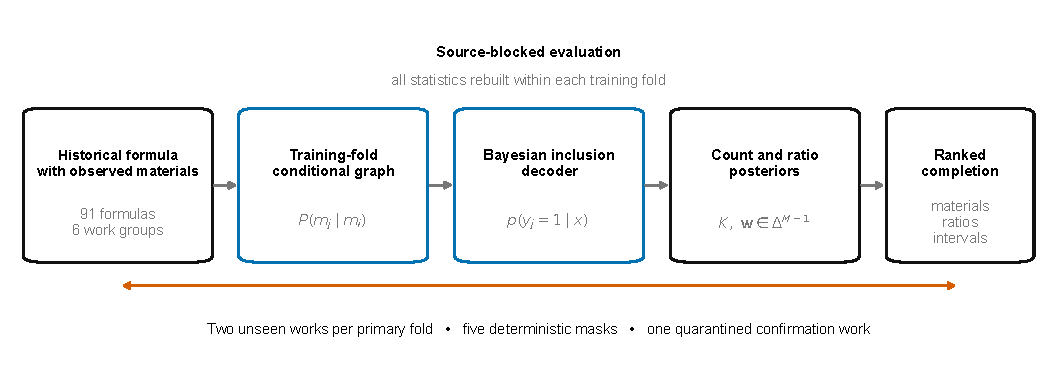
\includegraphics[width=\textwidth,height=0.78\textheight,keepaspectratio]{figures/fig1_workflow.pdf}

\caption{Xiangji-CGIR workflow and evaluation design. Historical formulas supply titles, source identifiers and deterministically observed material subsets. A training-fold directed material graph generates candidate affinities. A Gaussian-prior logistic decoder produces inclusion probabilities, after which count and ratio posteriors define a ranked completion with intervals. Every statistic is rebuilt within the training fold. The primary design holds out two entire work groups per fold and uses five deterministic masks; the Hong work is reserved for confirmation.}

\end{figure}

\begin{figure}[p]

\centering

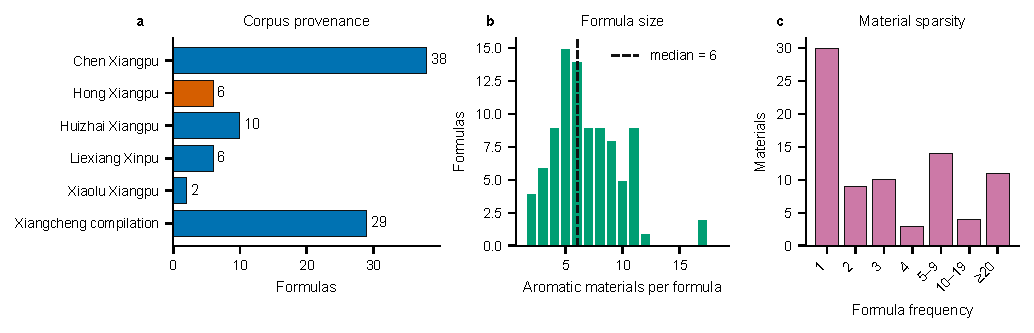
\includegraphics[width=\textwidth,height=0.78\textheight,keepaspectratio]{figures/fig2_corpus.pdf}

\caption{Corpus composition. \textbf{a}, Formula count by historical work group. Vermillion marks the six-formula Hong confirmation work; blue marks the five development and primary work groups. \textbf{b}, Distribution of aromatic material count across all 91 formulas; the dashed line marks the median of six. \textbf{c}, Number of canonical materials by corpus formula frequency. Thirty of 81 materials occur once.}

\end{figure}

\begin{figure}[p]

\centering

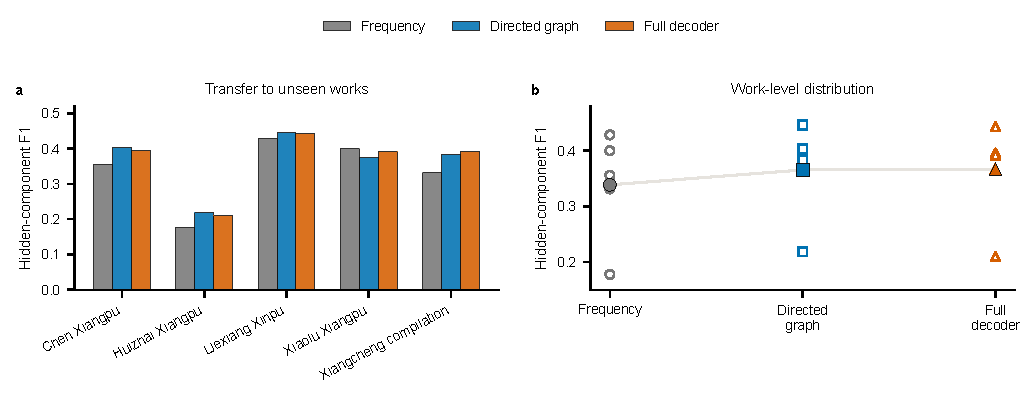
\includegraphics[width=\textwidth,height=0.78\textheight,keepaspectratio]{figures/fig3_primary_performance.pdf}

\caption{Primary source-shifted completion performance. \textbf{a}, Hidden-component F1 by held-out work group for global frequency, directed graph and the locked full decoder at 50\% observed context. Values average all source-pair appearances and five deterministic masks for each formula. \textbf{b}, Work-level values and source-macro means. Open markers show the five work groups; filled markers show their unweighted mean. Work groups form the unit of inference; repeated formula-mask instances do not.}

\end{figure}

\begin{figure}[p]

\centering

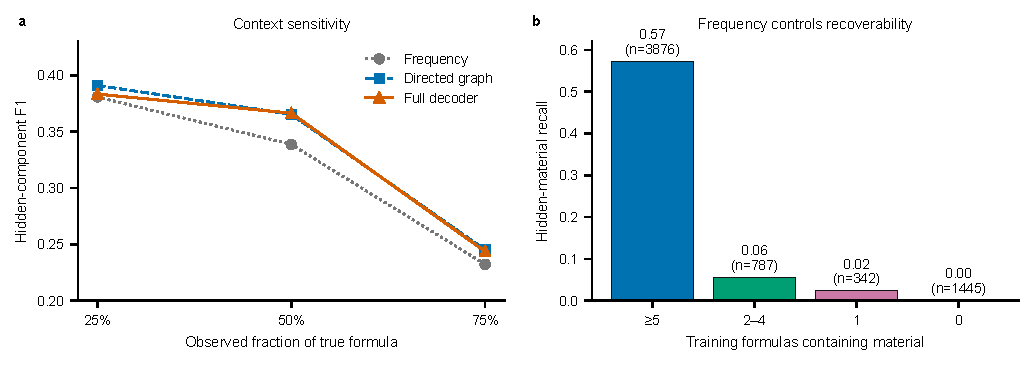
\includegraphics[width=\textwidth,height=0.78\textheight,keepaspectratio]{figures/fig4_robustness.pdf}

\caption{Context and rarity sensitivity. \textbf{a}, Source-macro hidden-component F1 at 25\%, 50\% and 75\% observed formula context. Color, marker and line style redundantly encode the three models. \textbf{b}, Hidden-material recall for the locked decoder grouped by material frequency in the corresponding training folds. Labels report recall and the number of repeated recovery opportunities across source-pair folds and masks.}

\end{figure}

\begin{figure}[p]

\centering

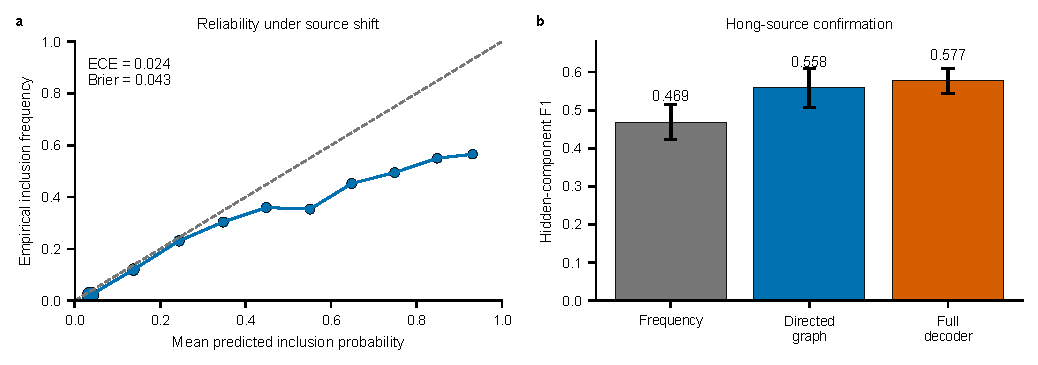
\includegraphics[width=\textwidth,height=0.78\textheight,keepaspectratio]{figures/fig5_uncertainty_confirmation.pdf}

\caption{Probabilistic behavior and confirmation. \textbf{a}, Ten-bin reliability curve for 95,210 hidden candidate decisions from the locked primary decoder. Marker area scales with the square root of bin count; the dashed diagonal marks exact calibration. \textbf{b}, Hidden-component F1 on six Hong-source formulas after model freeze. Bars show the mean across five deterministic masks and error bars show the standard deviation across masks. The confirmation formulas form one historical work group.}

\end{figure}

\begin{figure}[p]

\centering

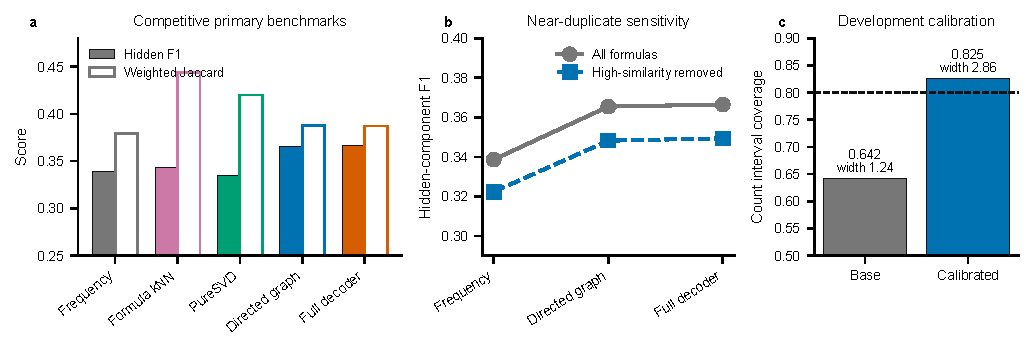
\includegraphics[width=\textwidth,height=0.78\textheight,keepaspectratio]{figures/fig6_stress_tests.pdf}

\caption{Competitive baselines and post-freeze stress tests. \textbf{a}, Source-macro hidden-component F1 and complete-composition weighted Jaccard for frequency, formula k-nearest neighbours, PureSVD, the directed graph and the full decoder. Formula-neighbour and PureSVD configurations were selected on development work splits. \textbf{b}, Hidden-component F1 before and after excluding nine formulas whose material-set Jaccard with another work group was at least 0.8. \textbf{c}, Primary coverage and mean width of the original count interval and the interval expanded by one material using work-held-out development residuals. The dashed line marks nominal 80\% coverage.}

\end{figure}

\clearpage

\end{document}
